\chapter{Adaptive Configuration Selection Method}  \label{chap:study}

In the considered system, the hydrophone configuration has a decisive role on the achieved precision as demonstrated. Therefore, a way to optimize the system's estimation would be to choose, for each position of the acoustic source, the configuration that returns the best estimation and thus the one that should be employed.

In a field scenario where a vehicle is searching for an acoustic transmitter, as it is navigating and readjusting its trajectory, the relative direction that is being estimated in real time is changing. Therefore, the system's performance can vary and arises the necessity of having a broader line of sight region from the hydrophones to the target. To resolve this issue, the proposed method assumes that the used USBL system integrates more than four hydrophones placed in known positions. This way, it is possible to reconfigure which four hydrophones are used at a time leading to an estimation that is the best possible for the available sensors (\textbf{RQ3}). 

This chapter is dedicated to explaining the methodological approach, the main findings and conclusions that were driven from the formulated optimal reconfiguration method. Firstly, the developed mechanism for defining line of sight regions for the deployed hydrophones is presented. Thereafter, the Monte Carlo method is explained, including the theoretical details as well as the developed algorithm. Then its functionality is demonstration through simulations that contemplate the three methods presented previously. Lastly, an adaptation to the method is made which selects an average optimal solution based on range. The performed simulations are presented and the obtained results are compared for each of the three evaluation methods previously explained.

\section{Line of Sight Definition} \label{subsec:lineofsight}

As briefly explained before, when considering a set of hydrophones placed in the surface of an AUV, there will be blind regions for each of the hydrophones. Nonetheless, when an acoustic source is positioned in a blind region of an hydrophone, it still can receive a transmitted signal through reflections on path objects or reverberation in the AUV's surface. Since these signals would be distorted from the original, they could lead to misinformation after the processing if they were to be considered. For this reason, it is essential to exclusively consider configurations whose hydrophones have line of sight (LOS) to the transmitter. 

In the present application, this feature is executed through function $line\_of\_sight$ of algorithm \ref{alg:alg2}, which outputs a vector containing all the hydrophones that have line of sight to the inputted transmitter position, $mean\_estimate$, from the considered set $matrix_{r_{i}}$. 

In order to define which hydrophones have LOS to a specific position in space, a region was defined for each hydrophone as its LOS region, $ls_i$. Thus, three simplifications were initially considered: 
\begin{itemize}
	\item The model for the vehicle is an approximation to a typical shape of an AUV using geometric shapes, as represented in \ref{fig:auv-geo}, composed by a cylinder as the body with $2*w$ of diameter and a cone in the front with height equal to $q$;
	
	\begin{figure}[!htbp]
		\makebox[\textwidth][c]{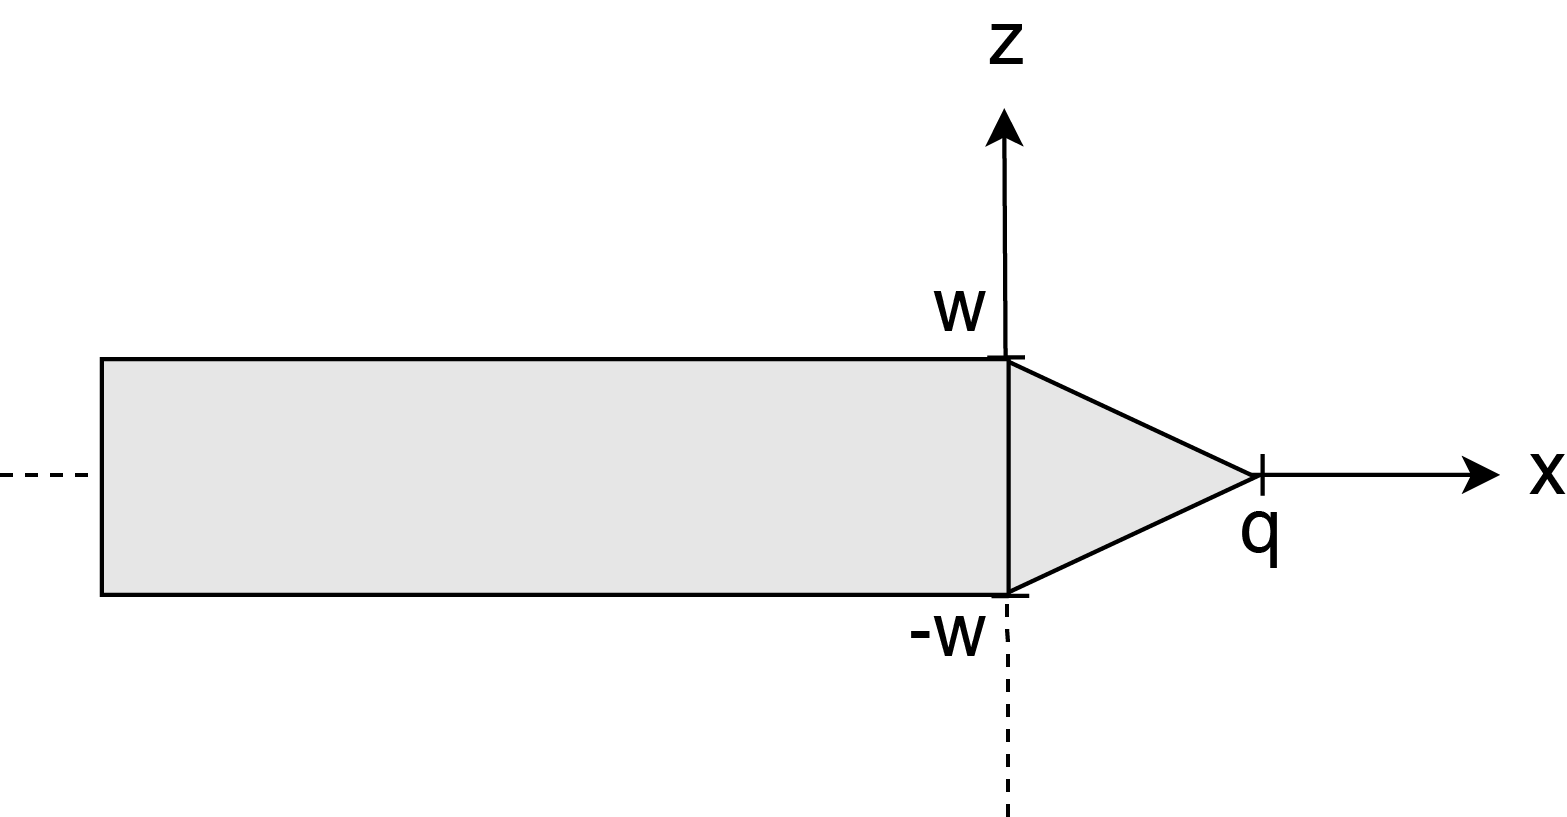
\includegraphics[width=0.4\textwidth]{figures/auv-geo}}
		\captionsetup{justification=centering,margin=2cm}
		\caption{Model of AUV used to calculate the LOS region}
		\label{fig:auv-geo}
	\end{figure}
	
	\item The regions for a $x \leq 0$ are defined as if the hydrophones were flat in the vehicle's surface, which leads to a simplified definition of the LOS region;
	
	\item Since hydrophone $r_1$ is integrated in every configuration, there is no necessity of defining its LOS region.
	
\end{itemize}

Having these relations into account, the LOS regions are then defined separately for $x \leq 0$ and $x > 0$. When $x \leq 0$, the second simplification previously mentioned is applied so all $ls_i$ are defined as the region greater/less or equal than the tangential to the position of hydrophone $i$ in plane yz. These tangential equations are defined in (\ref{eq:los-s2}) to (\ref{eq:los-s9}).

\begin{eqnarray}
	ls_2 \gets x \leq 0 \; \;  \wedge  \; \; z > r_{2_z} 
	\label{eq:los-s2} \\
	ls_3 \gets x \leq 0 \; \;  \wedge  \; \; z < r_{3_z} 
	\label{eq:los-s3} \\
	ls_4\gets x \leq 0 \; \;  \wedge  \; \; y > r_{4_y}
	\label{eq:los-s4} \\
	ls_5\gets 	x \leq 0 \; \;  \wedge  \; \; y < r_{5_y}
	\label{eq:los-s5} \\
	ls_6 \gets	x \leq 0 \; \; \wedge  \; \; z \; \geq \; - y + w \sqrt{2}
	\label{eq:los-s6} \\
	ls_7 \gets	x \leq 0 \; \; \wedge  \; \; z \; \leq \; y - w \sqrt{2}
	\label{eq:los-s7} \\
	ls_8 \gets x \leq 0 \; \; \wedge  \; \;  z \; \geq \; y + w \sqrt{2}
	\label{eq:los-s8} \\
	ls_9 \gets 	x \leq 0 \; \; \wedge  \; \;  z \; \leq \; - y - w \sqrt{2}
	\label{eq:los-s9}
\end{eqnarray}

By evaluating these equations, it is possible to infer that the LOS regions for $x \leq 0$ intersect each other, as illustrated in figure \ref{fig:los-color-s0}. The projection is correspondent to the yz plane with an inverted y-axis, in accordance with the previously presented model of the USBL system. Additionally, each colored line corresponds to the LOS region covered by the hydrophone with the same color. For instance, if a transmitter is located in $s_{cart}(-10,-10,-10)$, by analysis of the schematic it is observable that this position is covered by $ls_3$, $ls_5$ and $ls_9$, thus in line of sight of hydrophones 3,5 and 9.

\begin{figure}[!htbp]
	\makebox[\textwidth][c]{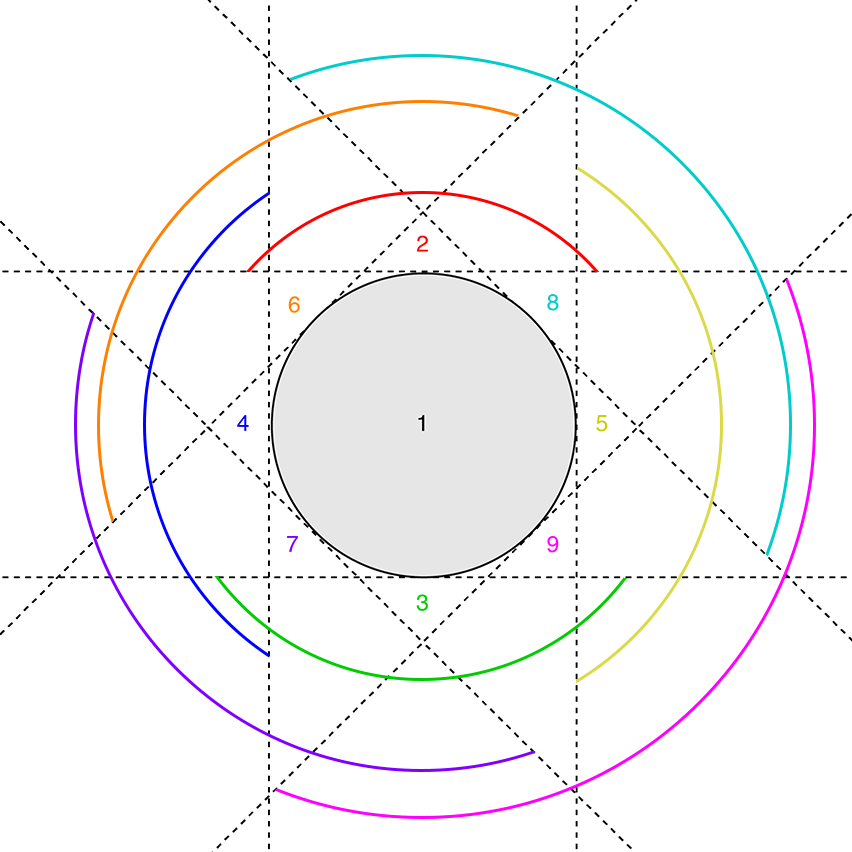
\includegraphics[width=0.6\textwidth]{figures/los-color-regions-back-crop}}
	\captionsetup{justification=centering,margin=2cm}
	\caption{Line of sight regions in plane yz for x < 0}
	\label{fig:los-color-s0}
\end{figure}

Analogously, when $x > 0$, all $ls_i$ are defined as the region greater/less or equal than the tangential to the position of hydrophone $i$ in planes xz or xy, depending on the hydrophone's location. Dealing with the hydrophones positioned in the y and z-axis, $r_2$, $r_3$, $r_4$ and $r_5$, it is possible to directly formulate equations that help defining $ls_2$, $ls_3$, $ls_4$ and $ls_5$ since the tangent plane to these hydrophones is perpendicular to referential planes. However, when considering hydrophones $r_6$, $r_7$, $r_8$ and $r_9$, which are not positioned in any referential axis, the tangential plane which passes through the hydrophone and the front limit of the cone is not parallel to any of the referential planes xy, xz or yz. Therefore, the equations that could define these planes require a rotation of the referential axis. In order to counter this issue, since the shape of the model projected in the yz plane is a circle , if hydrophones $r_6$, $r_7$, $r_8$ and $r_9$ are rotated a $45^{\circ}$ angle around the x-axis, they can become coincident with the positions of $r_2$, $r_4$, $r_5$ and $r_3$ respectively. Additionally, when considering this rotation, the position of the transmitter would also be rotated the same angle to maintain their relative positions. Overall, the used equations are defined by relations (\ref{eq:los-b2}) to (\ref{eq:los-b5}), where the regarded $x,y,z$ coordinates are the original transmitter position for $ls_2$, $ls_3$, $ls_4$, $ls_5$, and the rotated transmitter position for $ls_6$, $ls_7$, $ls_8$, $ls_9$.

\begin{eqnarray}
	ls_2, \;  ls_6  \gets x > 0 \; \;  \wedge  \; \; z \geq -\frac{w}{q} x + w  
	\label{eq:los-b2} \\
	ls_3, \;  ls_9 \gets x > 0 \; \;  \wedge  \; \; z \leq \frac{w}{q} x - w  
	\label{eq:los-b3} \\
	ls_4, \;  ls_7 \gets x > 0 \; \;  \wedge  \; \; y \geq -\frac{w}{q} x + w 
	\label{eq:los-b4} \\
	ls_5, \;  ls_8 \gets x > 0 \; \;  \wedge  \; \; y \leq \frac{w}{q} x - w  
	\label{eq:los-b5}
\end{eqnarray}

After evaluating these equations and the limiting planes that they form, the projected regions of LOS for $r_2$, $r_3$, $r_4$ and $r_5$ are illustrated in \ref{fig:los-color-b0}, where their intersection is evident. The regions $ls_2$, $ls_3$, $ls_4$ and $ls_5$ are naturally similar to these, with an additional rotation of $45^{\circ}$ around the x-axis.

\begin{figure}[!htbp]
	\makebox[\textwidth][c]{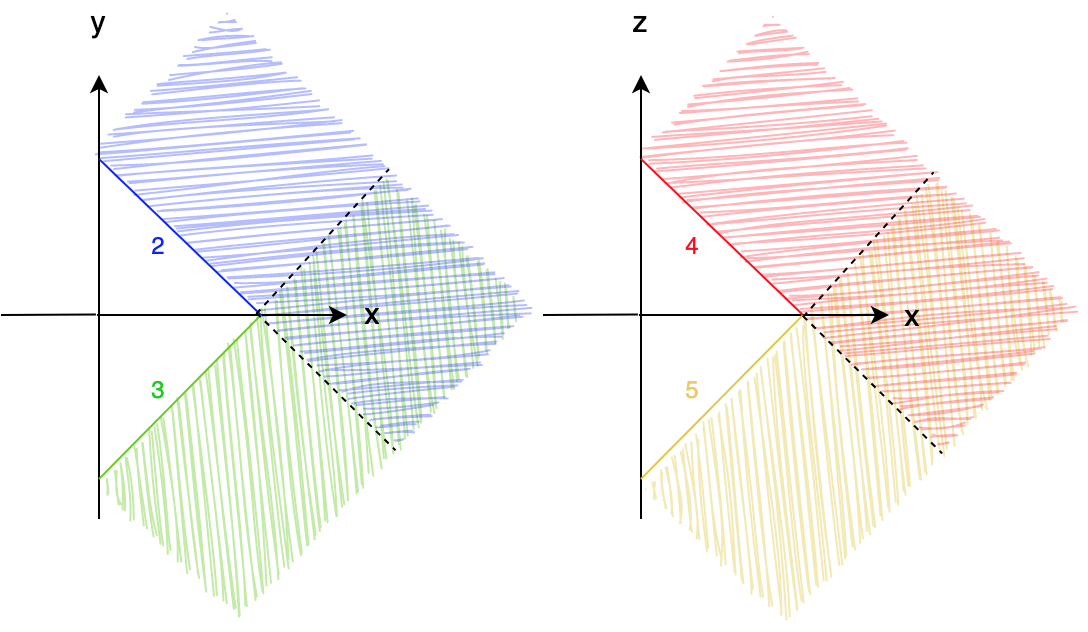
\includegraphics[width=0.7\textwidth]{figures/projections-los}}
	\captionsetup{justification=centering,margin=2cm}
	\caption{Line of sight regions in plane yx and zx for x $\geq$ 0}
	\label{fig:los-color-b0}
\end{figure}

In summary, it is possible to deduce that there is a larger quantity of different configurations that cover the space for $x>0$ than for $x \leq 0$ due to the model of the AUV and the considerations described in the course of this subsection. Therefore it is expected a better estimation for positions of the acoustic source with an azimuth angle between $-90^{\circ}$ and $90^{\circ}$.

\subsection{Practical Evaluation of the Line of Sight Regions}	

Upon inspecting the overall obtained results and the whole function of the system, a particular analysis is conducted on the mechanism that defines the hydrophones' LOS regions. As the estimation precision is not contemplated in this study, it is indifferent which estimation evaluation method is used for the simulations of this subsection. Therefore, all demonstrated results are performed with GBE.

The first position to be tested is $s(-10,-10,-10)$ which inherently has less hydrophones with line of sight, due to the method's limitation for $x \leq 0$. Additionally, since it is located in the seventh octant it is expected to be only in LOS with exactly three hydrophones, thus having only one available configuration with line of sight. After simulating, figure \ref{fig:errors-10-10-10} is obtained which verifies the concepts described. The only configuration with line of sight is number 30, composed by $r_1$, $r_3$, $r_5$ and $r_9$.

\begin{figure}[!htbp]
	\makebox[\textwidth][c]{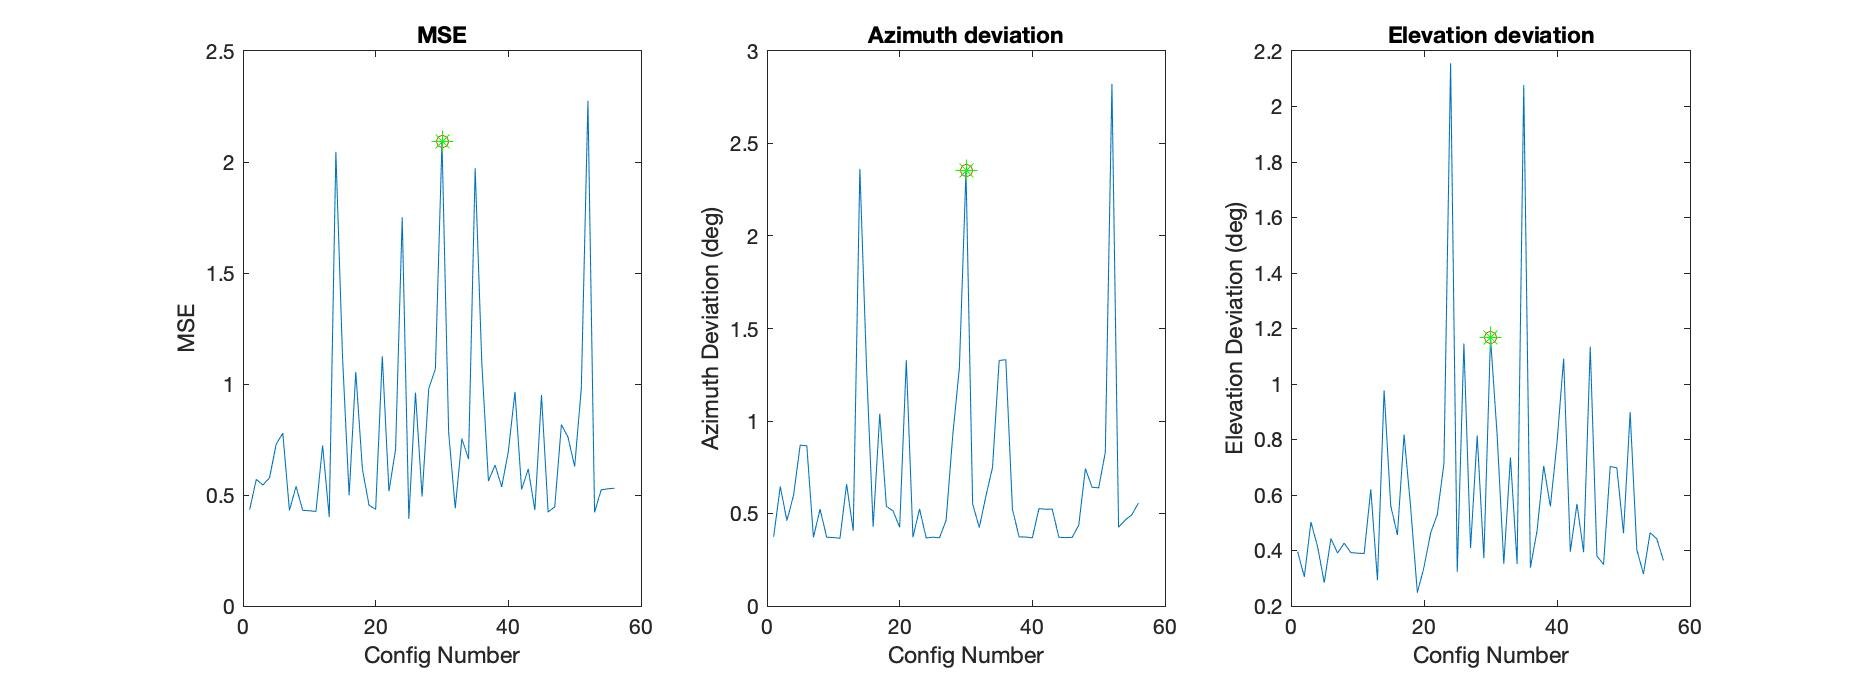
\includegraphics[width=1.3\textwidth]{figures/plot-[-10,-10,-10]-1000s-errors}}
	\captionsetup{justification=centering,margin=2cm}
	\caption{Errors obtained for all configurations when estimating position $s_{cart}(-10,-10,-10)$}
	\label{fig:errors-10-10-10}
\end{figure}

Then, position $s(100,0,0)$ is tested. Due to its long range location and the fact that it is assumed a conic shape at the front of the vehicle, it is expected that this point has line of sight for every employed hydrophone. Figure \ref{fig:errors-100-0-0} illustrates the simulated results which prove the theoretical expectation.

\begin{figure}[!htbp]
	\makebox[\textwidth][c]{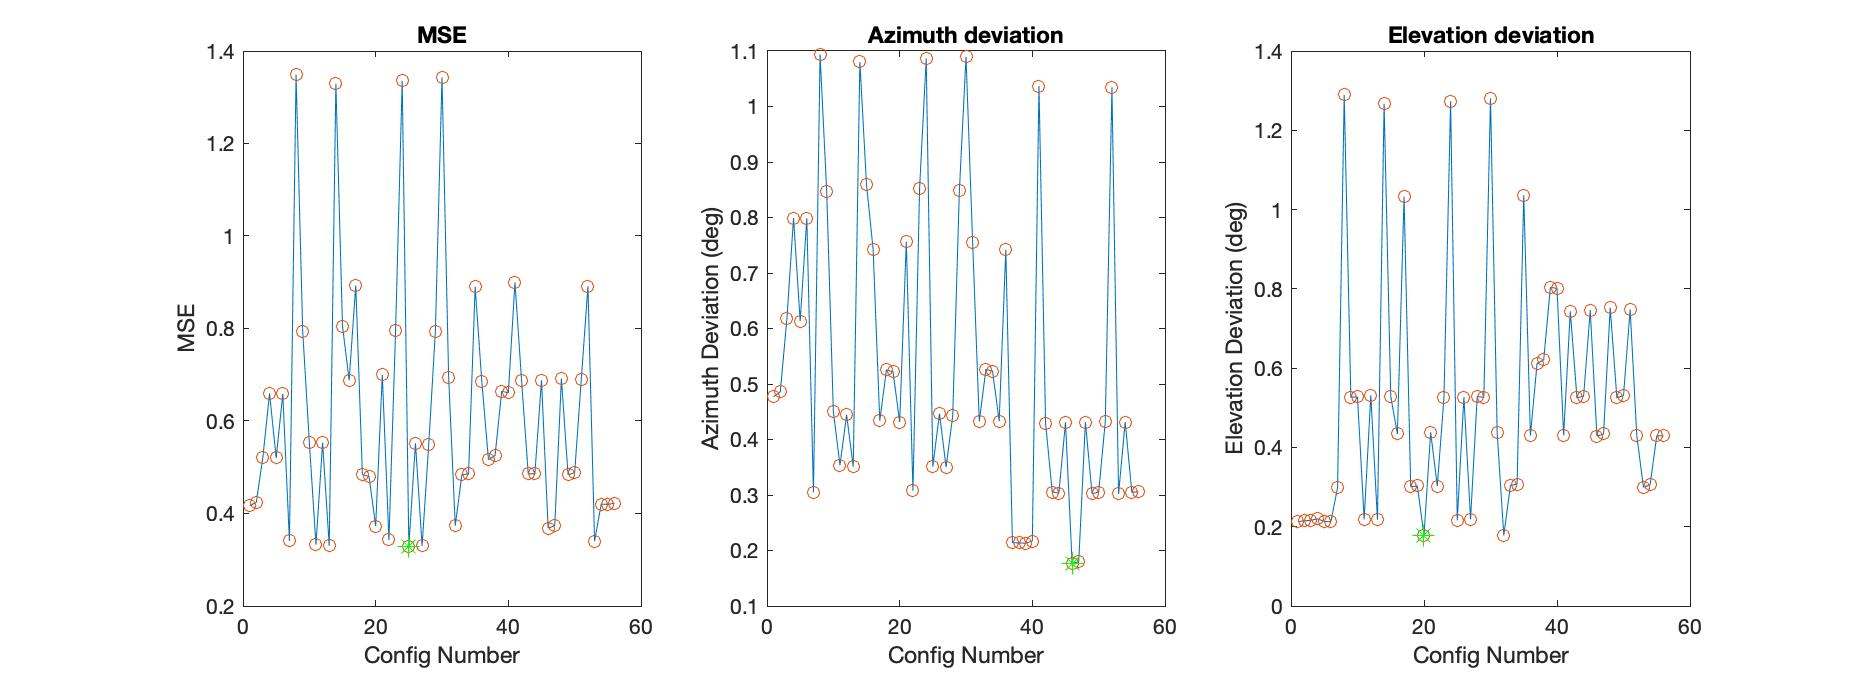
\includegraphics[width=1.3\textwidth]{figures/plot-[100,0,0]-1000s-errors}}
	\captionsetup{justification=centering,margin=2cm}
	\caption{Errors obtained for all configurations when estimating position (100,0,0)}
	\label{fig:errors-100-0-0}
\end{figure}

Lastly, an extensive verification process was held in order to ensure that the returned LOS hydrophones were plausible for many other positions. Table \ref{tab:LOS-var-pos} summarizes this search, containing a total of eleven positions spread over each octant and the reference axis. By consulting the hydrophone map illustrated in \ref{fig:9h-config}, it is possible to confirm that for every selected position the returned hydrophones are the logically expected.

\begin{table}[!htbp] %use H to adjust
	\begin{center}
		\begin{tabular}{ c c c c | c }
			\toprule
			\multicolumn{1}{c|}{} & \multicolumn{1}{c}{$s_x$} & $s_y$ & $s_z$ & Hydrophones with LOS\\
			\midrule
			\multicolumn{1}{c|}{x-axis} & \multirow{1}{*}{100} & 0 & 0 & 2, 3, 4, 5, 6, 7, 8, 9 \\
			\midrule
			\multicolumn{1}{c|}{y-axis} & \multirow{1}{*}{0} & 100 & 0 & 4, 6, 7 \\
			\midrule
			\multicolumn{1}{c|}{z-axis} & \multirow{1}{*}{0} & 0 & 100 & 2, 6, 8  \\
			\midrule
			\multicolumn{1}{c|}{$1^{st}$ octant} & \multirow{1}{*}{10} & 10 & 10 & 2, 4, 6, 7, 8 \\
			\midrule
			\multicolumn{1}{c|}{$2^{nd}$ octant} & \multirow{1}{*}{5} & 5 & -1 & 2, 3, 4, 6, 7 \\
			\midrule
			\multicolumn{1}{c|}{$3^{rd}$ octant} & \multirow{1}{*}{1} & -1 & 0 & 2, 3, 5, 8, 9  \\
			\midrule
			\multicolumn{1}{c|}{$4^{th}$ octant} & \multirow{1}{*}{1} & -10 & -10 & 3, 5, 7, 8, 9 \\
			\midrule
			\multicolumn{1}{c|}{$5^{th}$ octant} & \multirow{1}{*}{-100} & 10 & 10 & 2, 4, 6  \\
			\midrule
			\multicolumn{1}{c|}{$6^{th}$ octant} & \multirow{1}{*}{-1 } & 10 & -5 & 3, 4, 6, 7  \\
			\midrule
			\multicolumn{1}{c|}{$7^{th}$ octant} & \multirow{1}{*}{-1} & -1 & 1 & 2, 5, 8 \\
			\midrule
			\multicolumn{1}{c|}{$8^{th}$ octant} & \multirow{1}{*}{-1} & -100 & -10 & 3, 5, 8, 9 \\
			\bottomrule 
		\end{tabular}
		\caption{Hydrophones with line of sight for several $s$ positions}
		\label{tab:LOS-var-pos}
	\end{center}
\end{table}


%----------------------------------------------------------------------------------------------------------------------------------------------------------

\section{Monte Carlo Approach} \label{sec:config-perf}

The developed algorithm serves as a tool to determine which is the best available hydrophone configuration for a certain target position. This approach uses a Monte Carlo method which is useful to solve problems that are deterministic in nature through repetition and application of random parameters. Additionally, it makes use of a selected performance evaluation method, detailed in \ref{chap:proposed_sys}. In the present section, all explanations contemplate the use of an estimator, however this is easily adaptable to be used with the FIM and other performance criteria.
		
For this experiment, a total of nine hydrophones is considered, whose positions are contained in $matrix_{r_{i}}$, defined by table \ref{tab:config-9h}. Each column expresses the coordinates of each hydrophone, $r_i$, where the value of $x_i$ is in the first row, the value of $y_i$ in the second row and the value of $z_i$ in the third row. Additionally, it is assumed $q = 0.1$, $w = 0.1$ and $e = \frac{ \sqrt{2}}{2} w$.

\begin{table}[!htbp] %use H to adjust
	\begin{center}
		\begin{tabular}{c | c c c c c c c c c}
			\toprule
			& r1 & r2 & r3 & r4	& r5 & r6 & r7 & r8	& r9 \\ \hline 
			\multirow{1}{0.5em}{x} 
			& q & 0 & 0 & 0 & 0 & 0 & 0 & 0 & 0\\
			\midrule 
			\multirow{1}{0.5em}{y} 
			& 0 & 0 & 0 & w & -w & e & e & -e & -e\\
			\midrule 
			\multirow{1}{0.5em}{z} 
			& 0 & w & -w & 0 & 0 & e & -e & e & -e \\
			\bottomrule 
		\end{tabular}
		\caption{Position coordinates for the implementation using 9 hydrophones}
		\label{tab:config-9h}
	\end{center}
\end{table}

The presented hydrophone distribution was selected with no evidence of being superior to other possibilities and it tries to expand the traditional tetrahedral deployment, attending to the geometric characteristics of a torpedo-shaped AUV. The positions arrangement are represented in figure \ref{fig:9h-config}, where hydrophone $r_1$ is placed in front of the vehicle and hydrophones $r_2$ to $r_9$ form a circle with a $w$ meters radius around the vehicle.

\begin{figure}[!htbp]
	
	\makebox[\textwidth][c]{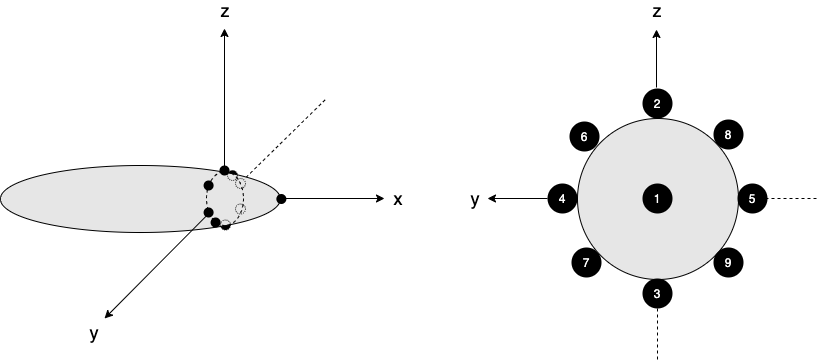
\includegraphics[width=0.9\textwidth]{figures/9h-config}}
	\captionsetup{justification=centering,margin=2cm}
	\caption{Hydrophone positions for the implementation using 9 hydrophones}
	\label{fig:9h-config}
\end{figure}

Since the used configuration has to be non coplanar, it is defined that hydrophone $r_1$ integrates all the configurations, constituted by sets of four hydrophones, as it is the only one that covers a third dimension. Accordingly, the number of configuration possibilities is combinations of three out of eight, $C(8,3)$, making up a total of 56. Each of these configurations are associated with a number from 1 to 56 and the hydrophones that integrate each of them are outlined in table \ref{tab:long} for consultation when necessary.

Having the system presented, the algorithm will be explained next. For the sake of clarity, the algorithm was outlined in pseudo code and separated into two main parts, where \ref{alg:alg1} is integrated in \ref{alg:alg2}.

\begin{algorithm}
	\setstretch{1.3} 	%increase space between lines
	%\algsetup{linenosize=\scriptsize} 	%adapts font size
	\scriptsize		%makes it smaller, idk
	\caption{Determines the average azimuth errors, elevation errors and MSE for a set of hydrophone configurations}
	\label{alg:alg1}
	\begin{algorithmic}[1]
		\FOR{\texttt{all k configurations}} %k = 1 \textbf{to} n\_config
		\FOR{\texttt{all i estimation repetition}} %i = 1 \textbf{to} accum\_samples
		\STATE\texttt{$estimator(s, config(k), error)$}
		\COMMENT{returns estimate in Cartesian and spherical coordinates}
		\STATE \texttt{accum\_estimate(i) $\gets$ result of the estimator in each repetition} 
		\STATE \texttt{accum\_error\_azimuth(i) $\gets$ azimuth error in each repetition} 
		\STATE \texttt{accum\_error\_elevation(i) $\gets$ elevation error in each repetition} 
		\ENDFOR
		\STATE $mean\_estimate \gets \dfrac{accum\_estimate}{accum\_samples}$
		\STATE
		\STATE $deviation\_azimuth(config) = std(accum\_error\_azimuth);$
		\STATE $deviation\_elevation(config) = std(accum\_error\_elevation);$
		%\newline
		\STATE $error\_azimuth(config) = mean(accum\_error\_azimuth);$
		\STATE $error\_elevation(config) = mean(accum\_error\_elevation);$
		\STATE
		\STATE $mse(config) = \sqrt{\rule{0pt}{8pt}error\_azimuth(config)^{2} + error\_elevation(config)^{2}};$
		\ENDFOR
	\end{algorithmic}
\end{algorithm}

Algorithm \ref{alg:alg1} is dedicated to computing the average azimuth error, elevation error and MSE for each of the $k = 56$ hydrophone configuration, in order to understand which of them achieves the minimum deviations when estimating a specific position. In order to do so, for each possible hydrophone configuration, the chosen acoustic source position $s$ was estimated $i = 1000$ times (line 3), using the developed estimator. This includes an injected error to the TDoA that follows a Gaussian distribution with zero mean and a configurable variance of $\sigma^{2}$, i.e., $e_i \sim \mathcal{N}(0,\,\sigma^{2})$. The result of this repetition would be an estimate cloud around the absolute $s$ position, which indicates the estimation variation achieved by a certain configuration for a specific position in space. At each stage of the repetition, the estimate is accumulated and the errors of azimuth and elevation are calculated, similarly to the process described in \ref{subsec:perform-compar-meth}. Therefore, after computing all estimation repetitions, it is possible to extract four essential parameters that define the quality of the estimation for each configuration: a mean estimate (line 8); the azimuth and elevation standard deviations (lines 10 and 11); the azimuth and elevation estimation errors (lines 12 and 13); the MSE (line 15).

Finally, using the obtained parameters it is possible to determine three configurations that lead to the best estimation regarding MSE, azimuth deviation and elevation deviation. However, there are two main issues that this simple algorithm does not take into account:

\begin{enumerate}
	
	\item  For the considered system conditions, when testing the same position $s$ multiple times, different hydrophone combinations are returned as the best option, which is an inconsistency originated by introduced noise $e_i$.
	
	\item Assuming that the hydrophone system is deployed in an AUV, it is expected that every hydrophone has a blind spot, where the acoustic source can be located. Even though the transmitted signals could still be received by these hydrophones, they would be distorted and could lead to misinformation so they should not be considered. Consequently the hydrophones that do not have line of sight to the transmitter should be disregarded as well. 
	
\end{enumerate}

In order to resolve both these problems, a second part of logic was developed, which is translated in pseudo code \ref{alg:alg2}.

In order to turn this mechanism more robust and solve the first issue, it is considered that the experiment of algorithm 1 has to be reiterated a defined number of times to obtain coherent and conclusive answers. Having said this, algorithm \ref{alg:alg2} begins with a loop that reiterates $j = 10$ times the logic previously explained. Addressing the second issue, the \textit{line\_of\_sight} function (line 7) is called, serving as filter to determine which hydrophones have line of sight to the estimated position. The mathematical definitions and conditions included in this function as well as the inputs and outputs are better clarified in the next subsection \ref{subsec:lineofsight}. Thereafter, all configurations that have full line of sight to the transmitter are extracted. Meanwhile, the azimuth deviations, elevation deviations and MSE are accumulated in each experiment reiteration (line 8 to 10) so that it is possible to obtain the definitive mean of these parameters for each configuration (line 12 to 14). 

\begin{algorithm}
	\setstretch{1.3} 	%increase space between lines
	%\algsetup{linenosize=\scriptsize} 	%adapts font size
	\scriptsize		%makes it small, idk
	\caption{Determines the overall best configuration for a specific position estimation considering: \\- multiple full experiments (Algorithm 1); \\ - only hydrophones with line of sight to the target.}
	\label{alg:alg2}
	\begin{algorithmic}[1]
		\FOR{\texttt{all j experiment reiterations}} %j = 1 \textbf{to} n\_test
		\STATE {\texttt{**************************}}
		\STATE {\texttt{*** INSERT ALGORITHM 1 ***}}
		\STATE {\texttt{**************************}}
		\STATE
		\STATE $line\_of\_sight(mean\_estimate, matrix_{r_{i}})$
		\COMMENT{returns which hydrophones have line of sight to the transmitter}
		\STATE
		\STATE \texttt{$reit\_mse = reit\_mse + mse$ }
		\STATE \texttt{$reit\_dev\_azimuth = reit\_error\_azimuth + deviation\_azimuth$ } 
		\STATE \texttt{$reit\_dev\_elevation = reit\_error\_elevation + deviation\_elevation$} 
		\ENDFOR
		\STATE \texttt{$mean\_MSE = reit\_mse \div j$ }
		\STATE \texttt{$mean\_dev\_azimuth = reit\_dev\_azimuth \div j$ } 
		\STATE \texttt{$mean\_dev\_elevation = reit\_dev\_elevation \div  j$} 
		\STATE
		\STATE {\texttt{Extract the configurations that contain only hydrophones with line of sight}}  
		\STATE {\texttt{Form matrix with errors of only the configurations with full line of slight}}
		\STATE
		\STATE $[best\_config\_for\_mse,\; \; overall\_min\_mse] = min(overall\_mse)$
		\STATE $[best\_config\_for\_azimuth,\; \; overall\_min\_dev\_azimuth] = min(overall\_dev\_azimuth)$
		\STATE $[best\_config\_for\_elevation,\; \; overall\_min\_dev\_elevation] = min(overall\_dev\_elevation)$
	\end{algorithmic}
\end{algorithm}

At this stage, it is possible to know already which are the configurations that are considered to achieve the minimum errors in each $j$ reiteration and how many times each of them are chosen. However, these are still not filtered, thus they can contain occluded hydrophones, i.e. that do not have line of sight to the acoustic source. Consequently, the next step is to extract only the configuration with full LOS and form three matrices with the azimuth deviations, elevation deviations and MSE of these configurations. Having the final parameters calculated and filtered, the overall best configurations for each of the chosen parameters are given by the minimum of the matrices that contain said parameter (line 19 to 21), i.e. for all configurations with full LOS:

\begin{itemize}
	
	\item  The minimum obtained MSE corresponds to the configuration that more precisely estimates the position $s$ in terms of MSE;
	
	\item The minimum obtained azimuth deviation corresponds to the configuration that more precisely estimates the position $s$ in terms of azimuth;
	
	\item The minimum obtained elevation deviation corresponds to the configuration that more precisely estimates the position $s$ in terms of elevation.
	
\end{itemize}

Additionally, it is possible to obtain the best configuration in terms of azimuth and elevation simultaneously, by computing the mean between the deviation of azimuth and elevation in each of the selected configurations. The minimum value obtained corresponds to the configuration which achieve the minimum the deviation in both parameters simultaneously.

\section{Performance Comparison between Geometric Configurations } \label{sec:analysis_config_performance}
%
For the purpose of demonstrating the functionality of the developed adaptive configuration selection method, two types of simulations will be performed :

\begin{itemize}
	\item \textbf{Type SS (Specific Simulation)} that generates the estimation of a specific transmitter position using several configurations and compares the obtained estimation precision and best configuration by each of the three methods presented in chapter \ref{chap:proposed_sys}.
	
	\item \textbf{Type BS (Broad Simulation)} that generates the estimation of several positions with short and long ranges, that form spheres around the origin of the coordinate axes, for an increased number of configurations. Then the obtained best configurations for specific defined criteria are compared for the three methods presented in chapter \ref{chap:proposed_sys}.
	
\end{itemize}

Similarity to \ref{subsec:perform-compar-meth}, the evaluated criteria for the GBE and PWE are the achieved MSE, azimuth deviation and elevation deviation, whereas for the FIM the chosen optimality criteria is A-, D- and E-optimality. 

\subsection{SS Analysis}

The simulations run in this subsection evaluate the estimation precision achieved by the 56 configurations defined previously, for the specific transmitter position $s_{cart}(10,10,10)$. 

The plots that will be presented throughout the study show the metrics values for each configuration, highlighting the computed best configuration in each case. The plots can be interpreted as follows: 

\begin{itemize}
	\item The configurations marked with a red circle correspond to those whose hydrophones have line of sight to the transmitter;
	
	\item The green star indicates the configuration that achieves the lowest estimation error, i.e. the best configuration for the contemplated metric;
	
	\item When the azimuth and elevation deviations are evaluated simultaneously, the obtained plots are overlaid for a clear comparison between results, which can be interpreted as follows:
	
	\begin{itemize}
		\item The azimuth deviation in degrees is represented by the blue line;
		\item  The elevation deviation in degrees is represented by the pink line;
		\item The cyan diamond reveals which of the configurations leads to the minimum mean between the azimuth and the elevation deviations.
	\end{itemize}
	
\end{itemize}

When running this experiment for the GBE, plot \ref{fig:errors-101010} is obtained.For the present case, the hydrophones considered to have line of sight to the target are $r_2$, $r_4$, $r_6$, $r_7$ and $r_8$. The configuration with lowest MSE and azimuth deviation is number 8, composed by hydrophones $r_1$, $r_2$, $r_4$ and $r_6$, which are the directly closer to the target. The configuration that originates lowest elevation deviation is number 19, composed by $r_1$, $r_2$, $r_7$ and $r_8$, which maximizes the baseline of the sensors with line of sight. Additionally, figure \ref{fig:both-101010} represents the overlaid azimuth and elevation deviations obtained with the GBE. In this case, the best configuration corresponds to number 53 which reaches a mean deviation of $0.385^{\circ}$. 

\begin{figure}[!htbp]
	\makebox[\textwidth][c]{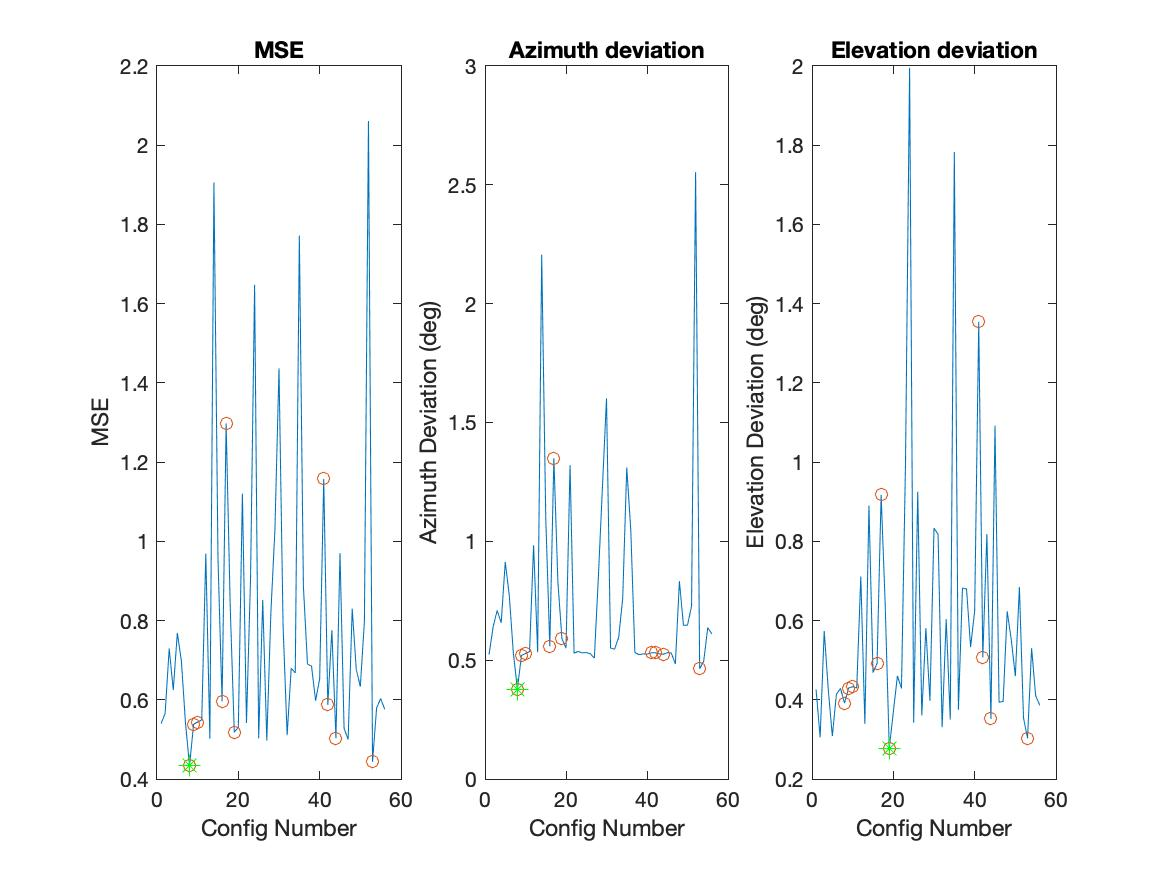
\includegraphics[width=1.3\textwidth]{figures/plot-[10,10,10]-1000s-errors}}
	\captionsetup{justification=centering,margin=2cm}
	\caption{Errors obtained for all configurations when estimating position $s_{cart}(10,10,10)$ using the GBE}
	\label{fig:errors-101010}
\end{figure}

\begin{figure}[!htbp]
	\makebox[\textwidth][c]{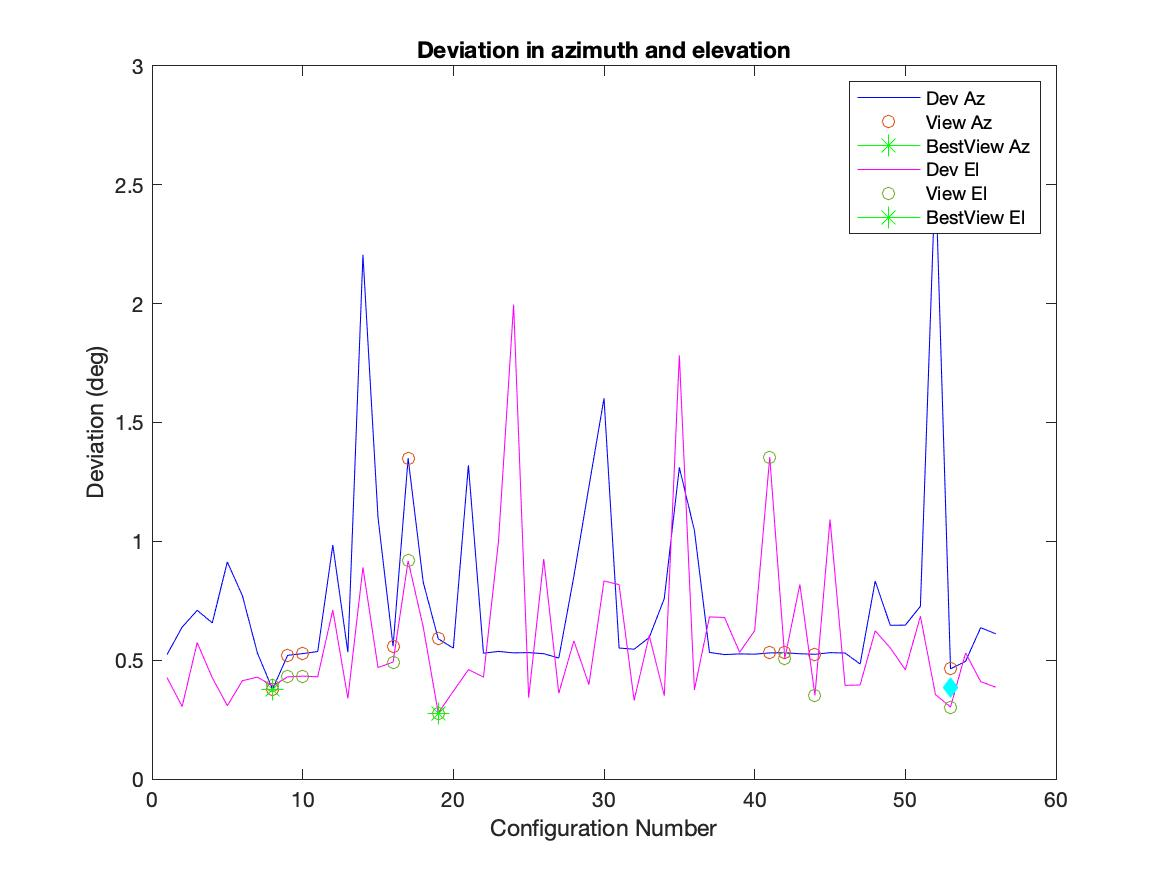
\includegraphics[width=1\textwidth]{figures/plot-[10,10,10]-1000s-both}}
	\captionsetup{justification=centering,margin=2cm}
	\caption{Overlaid azimuth and elevation deviations for all configurations when estimating position $s_{cart}(10,10,10)$ using the GBE}
	\label{fig:both-101010}
\end{figure}

Alternatively, the same experiment was done using the PWE. The results of the simulation show that the same set of hydrophones have line of sight to the transmitter, as expected. Plot \ref{fig:errors-101010-pseudo} corresponds to the obtained configurations' estimation precision. As can be observed the lowest MSE and azimuth deviation is number 53, which maximizes the baseline of the sensors with line of sight. The configuration that originates lowest elevation deviation is number 19, similarly to the observed result for the GBE. Additionally, figure \ref{fig:both-101010-pseudo} represents the overlaid azimuth and elevation deviations obtained with the PWE. In this case, the best configuration corresponds to number 53 which a mean deviation of $0.422^{\circ}$. 

\begin{figure}[!htbp]
	\makebox[\textwidth][c]{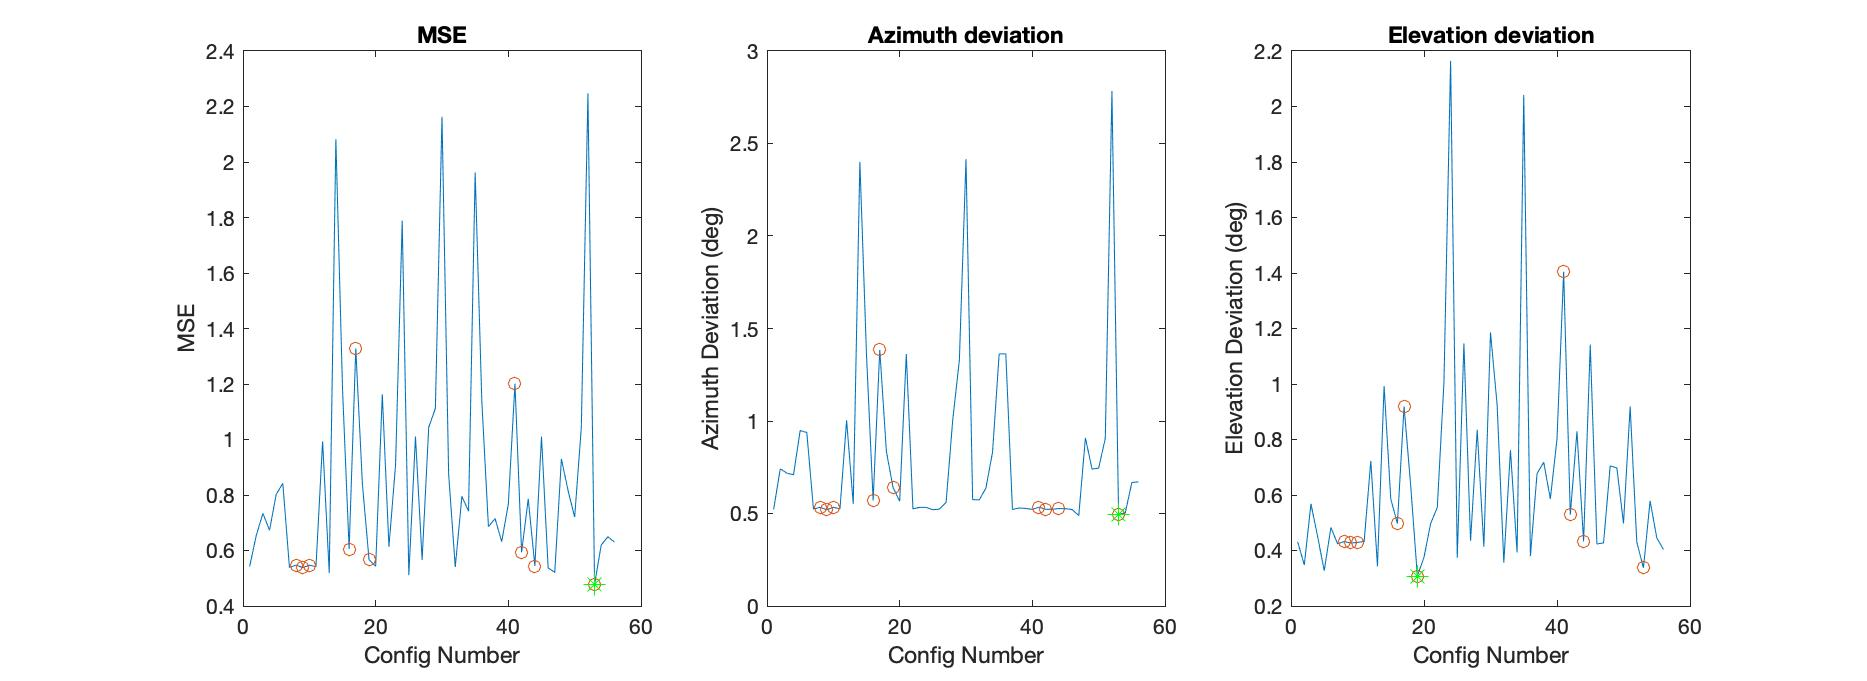
\includegraphics[width=1.3\textwidth]{figures/plot-[10,10,10]-1000s-errors-pseudo}}
	\captionsetup{justification=centering,margin=2cm}
	\caption{Overlaid azimuth and elevation deviations when estimating position $s_{cart}(10,10,10)$ using the PWE}
	\label{fig:errors-101010-pseudo}
\end{figure}

\begin{figure}[!h]
	\makebox[\textwidth][c]{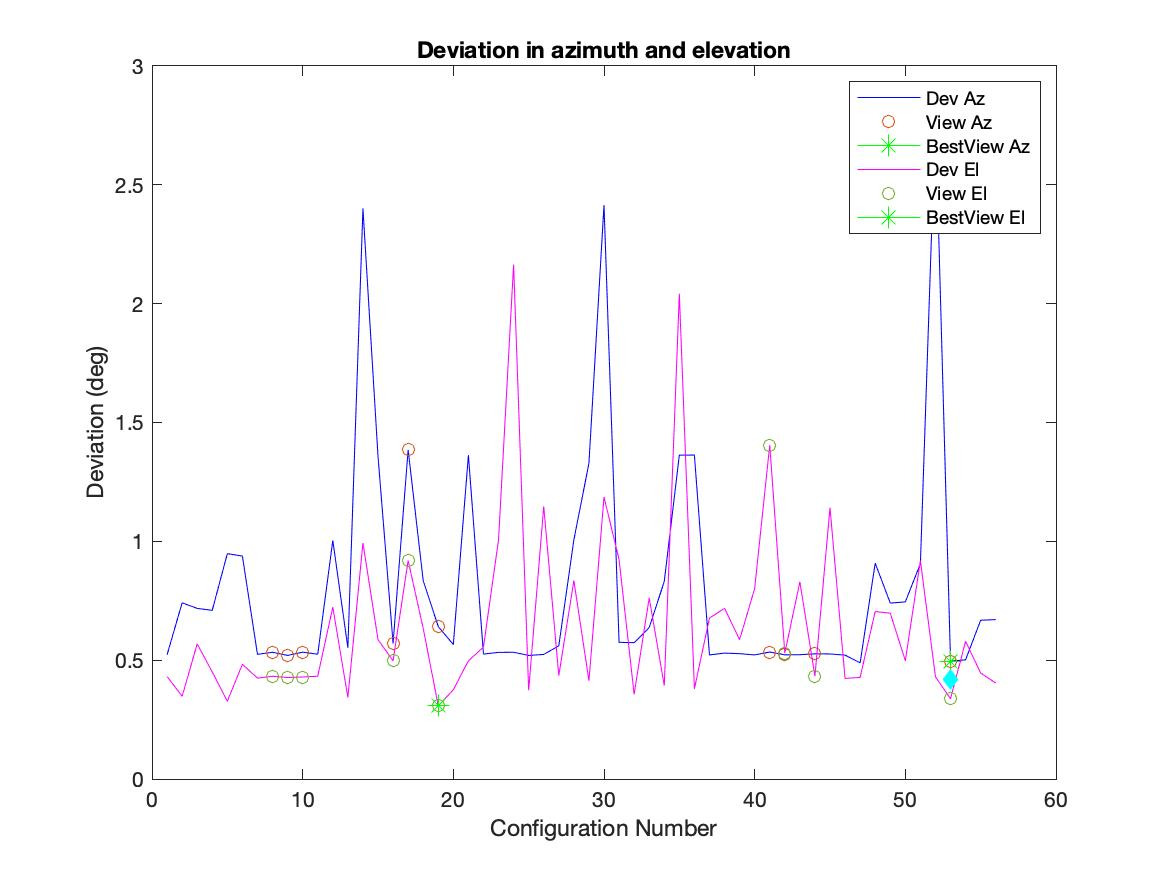
\includegraphics[width=1\textwidth]{figures/plot-[10,10,10]-1000s-both-pseudo}}
	\captionsetup{justification=centering,margin=2cm}
	\caption{Overlaid azimuth and elevation deviations when estimating position $s_{cart}(10,10,10)$ using the PWE}
	\label{fig:both-101010-pseudo}
\end{figure}

Finally, the same experiment was performed using the Crámer-Rao lower bound with the A-optimality, D-optimality and E-optimality. The obtained results are illustrated in \ref{fig:both-101010-fim}, which reveal matching best configurations with specific metrics for the GBE and the PWE. Accordingly, for the A- and D- optimality, configuration number 53 achieves the best estimation precision, with a summed uncertainty axis magnitude of $0.026m$ and uncertainty volume of $0.0164m^3$. For E-optimality, configuration number 8 is considered the most adequate achieving the minimum largest ellipsoid uncertainty axis among all configurations, with magnitude equal to $0.128m$.

\begin{figure}[!htbp]
	\makebox[\textwidth][c]{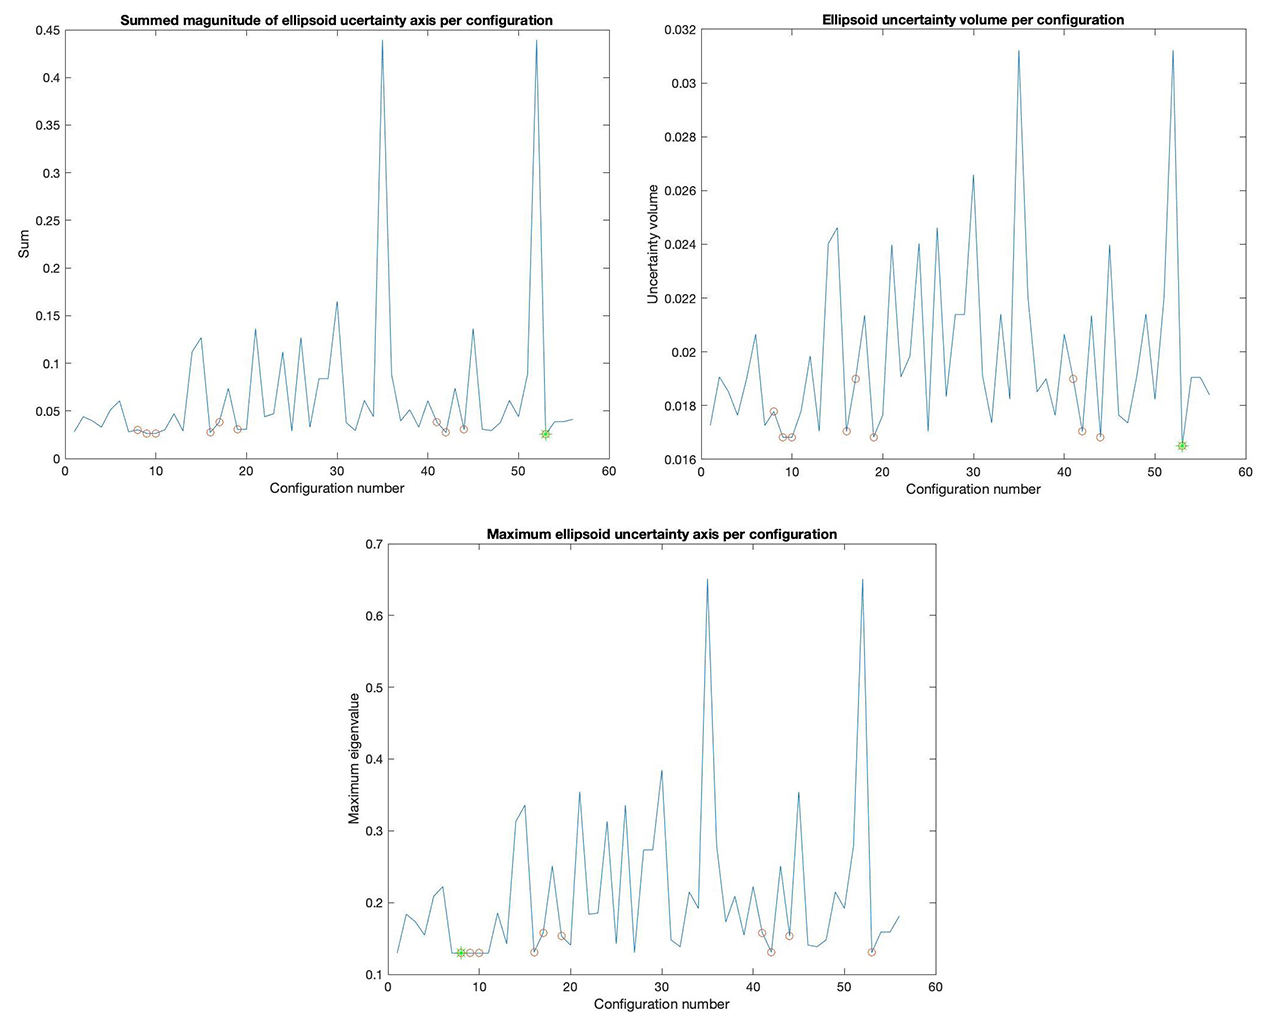
\includegraphics[width=1.1\textwidth]{figures/fim-plot-best-10,10,10}}
	\captionsetup{justification=centering,margin=2cm}
	\caption{Overlaid azimuth and elevation deviations when estimating position $s_{cart}(10,10,10)$ using the FIM}
	\label{fig:both-101010-fim}
\end{figure}

Upon investigating a specific position, several more individual positions were tested so that it would be possible to understand the behavior of the developed tool and generalize some of its characteristics. The main conclusions are summarized as follows:
\begin{itemize}
	\item Configurations that achieve the overall minimum errors tend to integrate the LOS hydrophones that attain among the larger distances between them, i.e. larger baseline;
	
	\item Transmitter positions that return a higher number of LOS hydrophones, have more possible configurations to choose from and therefore can be more optimized, presenting the lowest errors;
	
	\item The points directly behind the AUV, that cover positions with $y$ and $z$ in the range [-w,w], are not contained in any line of sight region. This results in a blind region for the formulated method, meaning that none of the hydrophones have line of sight to the transmitter. In such case, the signals may still be received with distortion, as mentioned in \ref{subsec:lineofsight}, decreasing the localization precision;
	
	\item When the transmitter positions have $x \leq 0$, they are in line of sight of less hydrophones than for $x > 0$, so there are fewer possible configurations and the returned best option for the various parameters are more consistent. Consequently, the returned minimum errors are usually higher than for $x > 0$;
	
	\item Transmitter positions that are located near the y-axis, almost in parallel with the circle of hydrophones, are usually covered by only four LOS regions, which correspond to the sensors that are directly closer to the target.
\end{itemize}

\subsection{BS Analysis} \label{subsec:bs-2}

After analyzing the outcome of the estimations of a specific transmitter position, an alternate scenario can be explored. In the present work, an effort is made to improve the localization precision for both short and long range, so it is useful to evaluate the performance of several configurations  not only for a single transmitter position but for the entire 3D space. 

Therefore, this series of broad simulations intend to derive which configurations demonstrate the best performance when estimating a set of positions placed along a sphere with defined radius centered at the origin. This way, it would be possible to determine which configurations, from a discrete set, perform on average the best for short and long range.

In order to test this approach, some adjustments were considered from the conditions established in the system used thus far:
\begin{itemize}
	\item It is assumed that the hydrophones are implemented in a structure that is invisible for the acoustic signals, thus all hydrophone positions have line of sight to any point in space;
	\item  The number of possible hydrophone locations is increased for a more extensive study.
\end{itemize}

Once again, hydrophone $r_1$ is integrated in all configurations and a total of 24 possibilities are considered for the remnant three. These include the same 8 positions $r_2$ to $r_9$, established for the initial setup in table\ref{tab:config-9h}, to which are added positions $r_{10}$ to $r_{25}$ defined in table \ref{tab:config-25h}. This addition corresponds to two replicated circles from the initial one, that assume the same $y$ and $z$ coordinates but are deviated from each other a $dx$ equal to 20 centimeters. Figure \ref{fig:24h-config} illustrates all the considered possible positions for the hydrophone's deployment. Accordingly, the number of possibilities is not correspondent to combinations of three out of 24, $C(24,3)$, since these contain non coplanar configurations. Therefore, the total number of available combinations to be tested is 1512.

\begin{table}[!htbp] %use H to adjust
	\begin{center}
		\makebox[\textwidth]{%
			\begin{tabular}{c | c c c c c c c c c c c c c c c c}
				\toprule
				& $r_{10}$ & $r_{11}$ & $r_{12}$ & $r_{13}$	& $r_{14}$ & $r_{15}$ & $r_{16}$ & $r_{17}$	& $r_{18}$ & $r_{19}$ & $r_{20}$ & $r_{21}$ & $r_{22}$ & $r_{23}$ & $r_{24}$ & $r_{25}$ \\ \midrule 
				\multirow{1}{0.5em}{x} 
				&$dx$&$dx$&$dx$&$dx$&$dx$&$dx$&$dx$&$dx$
				&$2dx$&$2dx$&$2dx$&$2dx$&$2dx$&$2dx$&$2dx$&$2dx$\\
				\midrule 
				\multirow{1}{0.5em}{y} 
				& 0 & 0 & w & -w & e & e & -e & -e
				& 0 & 0 & w & -w & e & e & -e & -e\\
				\hline 
				\multirow{1}{0.5em}{z} 
				& w & -w & 0 & 0 & e & -e & e & -e
				& w & -w & 0 & 0 & e & -e & e & -e \\
				\bottomrule 
		\end{tabular}}
		\caption{Additional coordinates for an implementation with 25 hydrophones}
		\label{tab:config-25h}
	\end{center}
\end{table}

\begin{figure}[!htb]
	\makebox[\textwidth][c]{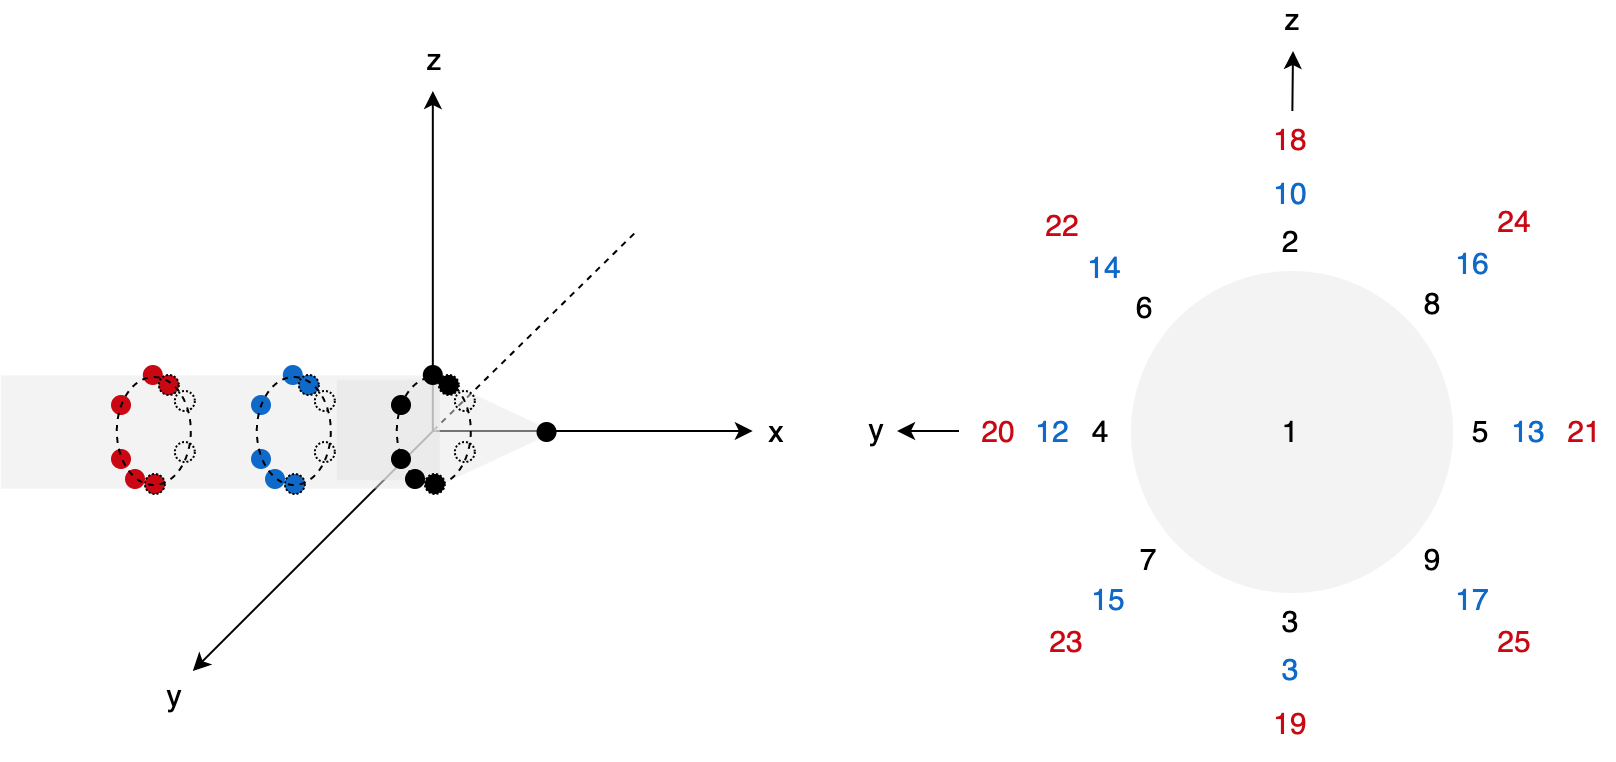
\includegraphics[width=0.9\textwidth]{figures/24h-config}}
	\captionsetup{justification=centering,margin=2cm}
	\caption{Hydrophone possible positions for optimality study based on range}
	\label{fig:24h-config}
\end{figure}

The applied algorithm is similar to the previously explained algorithms \ref{alg:alg1} and \ref{alg:alg2}, with the following variations:

\begin{enumerate}
		
	\item An additional logical loop is added in algorithm \ref{alg:alg1} between lines 1 and 2, so that for each possible configuration all $s$ are estimated a number of $i = 1000$ iterations.
	
	\item the $line\_of\_sight$ function is no longer used, as it is considered that all hydrophones have line of sight to every position $s$.
	
\end{enumerate}

The adapted algorithm was tested through a series of simulations, in which all 1512 defined configurations are used to estimate positions forming spheres of norms between $1m$ and $10000m$. In order to provide a more contextualized explanation of the subsequently simulation results, figure \ref{fig:config-images} is presented in advance, containing the most relevant representations that will be contemplated. This allows to visually associate the mentioned configuration numbers to the actual hydrophone placement throughout the following results description.

\begin{figure}[!htb]
	\makebox[\textwidth][c]{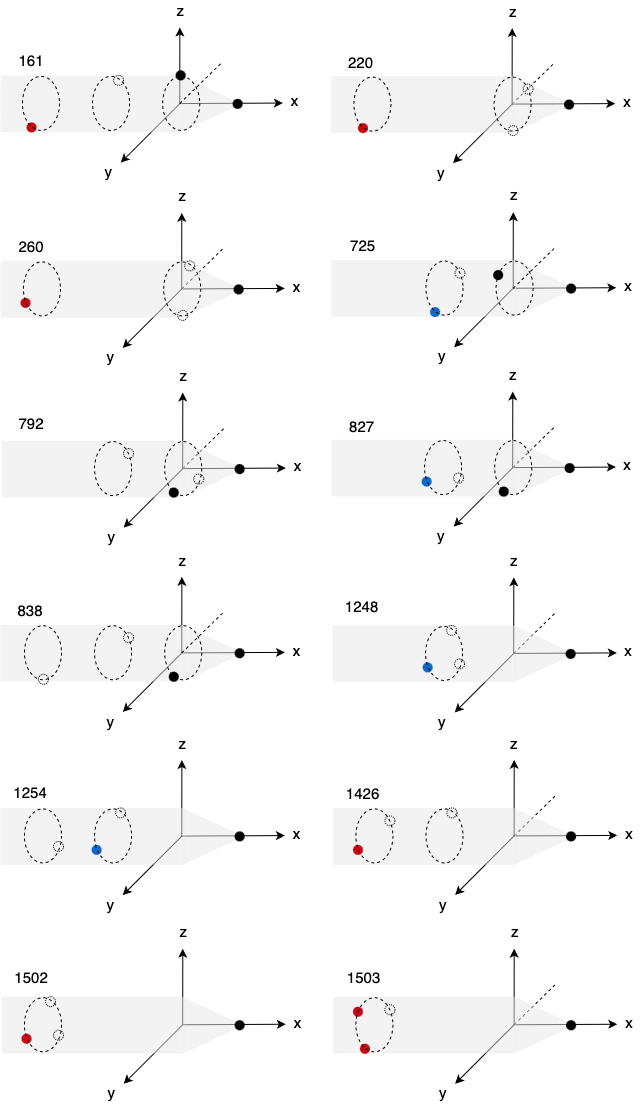
\includegraphics[width=0.8\textwidth]{figures/best-config-fim}}
	\captionsetup{justification=centering,margin=2cm}
	\caption{Illustration of relevant hydrophone configurations for range based estimation}
	\label{fig:config-images}
\end{figure}

Firstly, simulations are performed for the GBE and the collected data is summarized in table \ref{tab:montecarlo-best-all-gbe}.

\begin{table}[!htbp] %use H to adjust
	\begin{center}
		\makebox[\textwidth]{%
			\begin{tabular}{ c | c c | c c | c c | c c}
				\toprule
				\multicolumn{1}{c|}{\textbf{}} & 
				\multicolumn{2}{c|}{\textbf{Azimuth}} & \multicolumn{2}{c|}{\textbf{Elevation}} & \multicolumn{2}{c|}{\textbf{Azimuth+Elevation}} & 
				\multicolumn{2}{c}{\textbf{MSE}}  \\
				\midrule
				\multicolumn{1}{c|}{Norm} & Config & Min  & Config & Min & Config & Min & Config & Min \\
				\midrule
				\multirow{1}{*}{1} & 792 & 0.4730 & 220 & 0.1758 & 862 & 0.3554 & 862 & 0.4654\\
				\midrule
				\multirow{1}{*}{2} & 792 & 0.4771 & 220 & 0.1738 & 827 & 0.3905 & 827 & 0.4549 \\
				\midrule
				\multirow{1}{*}{3} & 792 & 0.4820 & 220 & 0.1752 & 827 & 0.3921 & 860 & 0.4571\\
				\midrule
				\multirow{1}{*}{10} & 792 & 0.4796 & 260 & 0.1702 & 827 & 0.3918 & 827 & 0.4572\\
				\midrule
				\multirow{1}{*}{20} & 827 & 0.4893 & 260 & 0.1702 & 827 & 0.3905 & 827 & 0.4537\\
				\midrule
				\multirow{1}{*}{50} & 792 & 0.4940 & 220 & 0.1705 & 860 & 0.3947 & 860 & 0.4615\\
				\midrule
				\multirow{1}{*}{100} & 860 & 0.4881 & 260 & 0.1707 & 827 & 0.3913 & 860 & 0.4538\\
				\midrule
				\multirow{1}{*}{200} & 827 & 0.4853 & 260 & 0.1706 & 827 & 0.3889 & 827 & 0.4511\\
				\midrule
				\multirow{1}{*}{500} & 792 & 0.4886 & 260 & 0.1722 & 929 & 0.3935 & 862 & 0.4606\\
				\midrule
				\multirow{1}{*}{1000} & 827 & 0.4846 & 260 & 0.1709 & 827 & 0.3899  & 827 & 0.4524\\
				\midrule
				\multirow{1}{*}{10000} & 792 & 0.4810 & 260 & 0.1724 & 862 & 0.3920  & 827 & 0.4554\\
				\bottomrule 
		\end{tabular}}
		\caption{Results of Monte Carlo simulation for range based estimation using GBE}
		\label{tab:montecarlo-best-all-gbe}
	\end{center}
\end{table}

The overall results do not exhibit a specific configuration to be the clear best in short or long range for the chosen parameters. For performance based on azimuth, configuration number 792 shows best results for norms between 1 and 10 meters. However, for longer range the results do not tend to a specific configuration, alternating between essentially three alternatives. Regarding performance based on elevation, configuration 220 is indicated as the best for short range of 1 and 3 meters, while for longer ranges going from 10 to 10000 meters, configuration 260 is the clear nominated. As can be observed in the illustration, these are structurally similar. When evaluating azimuth and elevation precision simultaneously or MSE, the results are not clear and many configurations are alternated, where number 827 stands out as the most frequently indicated. Overall, for an increasing norm there is no significant variation on the error magnitude, as expected.

Upon analyzing the GBE, a second experiment is run using the PWE. The collected data is summarized in table \ref{tab:montecarlo-best-all-pwe}.

\begin{table}[!htbp] %use H to adjust
	\begin{center}
		\makebox[\textwidth]{%
			\begin{tabular}{ c | c c | c c | c c | c c}
				\toprule
				\multicolumn{1}{c|}{\textbf{}} & 
				\multicolumn{2}{c|}{\textbf{Azimuth}} & \multicolumn{2}{c|}{\textbf{Elevation}} & \multicolumn{2}{c|}{\textbf{Azimuth+Elevation}} & 
				\multicolumn{2}{c}{\textbf{MSE}}  \\
				\midrule
				\multicolumn{1}{c|}{Norm} & Config & Min  & Config & Min & Config & Min & Config & Min \\
				\midrule
				\multirow{1}{*}{1} & 330 & 0.105 & 838 & 0.056 & 842 & 0.134 & 794 & 0.632 \\
				\midrule
				\multirow{1}{*}{2} & 330 & 0.321 & 838 & 0.106 & 1206 & 0.390 & 794 & 0.668 \\
				\midrule
				\multirow{1}{*}{3} & 330 & 0.528 & 838 & 0.150 & 725 & 0.397 & 531 & 0.644 \\
				\midrule
				\multirow{1}{*}{10} & 1426 & 0.522 & 838 & 0.183 & 725 & 0.395 & 1015 & 0.580 \\
				\midrule
				\multirow{1}{*}{20} & 725 & 0.537 & 1426 & 0.173 & 725 & 0.401 & 1254 & 0.539 \\
				\midrule
				\multirow{1}{*}{50} & 1426 & 0.528 & 161 & 0.178 & 1254 & 0.402 & 1254 & 0.494 \\
				\midrule
				\multirow{1}{*}{100} & 725 & 0.173 & 161 & 0.387 & 725 & 0.387 & 725 & 0.465\\
				\midrule
				\multirow{1}{*}{200} & 1426 & 0.519 & 161 & 0.176 & 725 & 0.397 & 725 & 0.483 \\
				\midrule
				\multirow{1}{*}{500} & 1426 & 0.529 & 1426 & 0.182 & 725 & 0.393 & 725 & 0.474 \\
				\midrule
				\multirow{1}{*}{1000} & 1426 & 0.502 & 161 & 0.181 & 1254 & 0.401 & 1254 & 0.483 \\
				\midrule
				\multirow{1}{*}{10000} & 1426 & 0.544 & 1426 & 0.183 & 1254 & 0.398 & 1254 &  0.478\\
				\bottomrule 
		\end{tabular}}
		\caption{Results of Monte Carlo simulation for range based estimation using PWE}
		\label{tab:montecarlo-best-all-pwe}
	\end{center}
\end{table}

For this case, there is also no clear best configurations for short and long range estimation regarding the chosen parameters. For the performance based on azimuth, configuration number 330 is indicated for short ranges between 1 and 3 meters, whereas for the remaining norms configuration number 1426 is the most frequently presented. For performance based on elevation, configuration number 838 is indicated for short ranges between 1 and 10 meters, while for greater norms the layout alternated between numbers 1426 and 161. For the remaining metrics, there is no clear trend on the indicated configurations, however numbers 725 and 1254 are the most frequently selected. In terms of error magnitude, the MSE presents a decreasing tendency with increasing norm, which is expected since for short range the approximation to a plane wavefront is not adequate. The remaining error magnitudes are approximated to the obtained data for GBE.

For the third experiment, the Crámer-Rao lower bound is used and the collected data is summarized in table \ref{tab:fim-best1}. In order to clarify the notation, the stated parameters Eigenvalue, Determinant and Trace are correspondent respectively to the magnitude of the largest uncertainty axis, the uncertainty volume and the summed magnitudes of the uncertainty axis of the indicated configurations.

\begin{table}[!htbp] %use H to adjust
	\begin{center}
		\makebox[\textwidth]{%
		\begin{tabular}{ c | c c | c c | c c }
			\toprule
			\multicolumn{1}{c|}{\textbf{}} & 
			\multicolumn{2}{c|}{\textbf{E-optimality}} & \multicolumn{2}{c|}{\textbf{D-Optimality}} & \multicolumn{2}{c}{\textbf{A-Optimality}} \\
			\midrule
			\multicolumn{1}{c|}{Norm} & Config & Eigenvalue  & Config & Determinant & Config & Trace \\
			\midrule
			\multirow{1}{*}{1} & 1248 & 6.2$\times10^{-3}$ & 1503 & 1.6$\times10^{-3}$ & 600 & 2.3$\times10^{-5}$ \\
			\midrule
			\multirow{1}{*}{2} & 1248 & 0.012 & 1503 & 2.5$\times10^{-3}$ & 1426 & 9.2$\times10^{-5}$  \\
			\midrule
			\multirow{1}{*}{3} & 1248 & 0.018 & 1503 & 3.3$\times10^{-3}$ & 1426 & 2.1$\times10^{-4}$  \\
			\midrule
			\multirow{1}{*}{10} & 1502 & 0.061 & 1503 & 7.4$\times10^{-3}$ & 1426 & 2.4$\times10^{-3}$ \\
			\midrule
			\multirow{1}{*}{20} & 1502 & 0.121 & 1503 & 0.012 & 1426 & 9.6$\times10^{-3}$\\
			\midrule
			\multirow{1}{*}{50} & 1502 & 0.303 & 1503 & 0.022 & 1426 & 0.061   \\
			\midrule
			\multirow{1}{*}{100} & 1502 & 0.606 & 1503 & 0.034 & 1426 & 0.242 \\
			\midrule
			\multirow{1}{*}{200} & 1502 & 1.212 & 1503 & 0.054 & 1426 & 0.968  \\
			\midrule
			\multirow{1}{*}{500} & 1502 & 3.029 & 1503 & 0.100 & 1426 & 6.055  \\
			\midrule
			\multirow{1}{*}{1000} & 1502 & 6.059 & 1503 & 0.159 & 1426 & 24.226 \\
			\midrule
			\multirow{1}{*}{10000} & 1502 & 60.587 & 1503 & 0.737 & 1426 & 2.42$\times10^{3}$ \\
			\bottomrule 
		\end{tabular}}
		\caption{Results of FIM simulation for range based estimation}
		\label{tab:fim-best1}
	\end{center}
\end{table}

By inspection, it is possible to observe that for each criterion there is a clear trend for the selected best configurations for short and long range, contrarily to most metrics of the previous results for GBE and PWE. Therefore, in terms of E-optimality configuration, an approximately constant error of 0.6\% is visible, where number 1248 shows the best performance for short range between 1 and 3 meters, while for long range from 10 to 10000 meters configuration 1502 is indicated. For D-optimality, a single configuration, number 1503, was considered the best for all defined ranges, which corresponds to an hydrophone placement that maximizes the baseline as illustrated in \ref{fig:config-images}. Finally, in terms of A-optimality configuration number 600 is indicated for norm equal to 1 meters and, for the remaining ranges, number 1426 is chosen as the best option.

As mentioned before, the FIM method is considered the most reliable method, as it does not depend on the selected estimator, and the results it presents demonstrate the most coherent configuration selection since it is a deterministic approach.
It should be noticed that for all obtained results configuration number 1426 is coincident between the PWE and the FIM simulations, which leads to believe that it comprises favorable characteristics to an increased localization precision. However, as the E-optimality optimizes a more relevant optimization criteria, it is expected that configuration number 1502 demonstrates even better results. 


\section{Summary and Discussion}

This chapter focuses on presenting the formulated adaptive configuration selection method, whose goal is to establish the sensor configuration that leads to the best estimation precision for a specific target position. After analyzing the results, it has proven to provide improved estimation precision by always selecting a configuration with line of sight to the target that achieves the lower estimation error. 

An adaptation to this method is also explored in \ref{subsec:bs-2}, whose goal is to select the sensor configuration that achieves the average best estimation for any target position along a sphere of defined norm. This allows to define optimal configurations based on the range, as demonstrated through simulations. As observed previously, the results of the Crámer-Rao lower bound demonstrate distinct optimal configurations for each optimality criteria in both short and long range. 

This mechanism could be applied to a data muling scenario, as established in chapter \ref{chap:intro}. If a discrete set of hydrophones are deployed in an mule AUV, then it is possible to adapt the selected configuration depending on the perceived angle of arrival in real-time. This would allow to always use the configuration that leads to the lower estimation error and thus improve the localization precision. 

Additionally, in a scenario where it is only relevant to have an average best estimation for both short and long range positions, then two configurations could be selected to be deployed. From the simulation results, considering the E-optimality as the most relevant criterion for this application, we can deduce that, for short range estimation, configuration number 1248 would be optimal, whereas, for long range, number 1502 would be preferred (\textbf{RQ4}).

Although configuration number 1502, illustrated in \ref{fig:config-images}, does not present the absolute best performance for positions in the entire 3D space, it obtains sufficiently satisfactory results in general to be considered an adequate option for both short and long range estimation. Therefore, for this specific configuration using a norm of $1000m$, it is possible to estimate that using the GBE, the approximated maximum expected deviation for azimuth is $2^{\circ}$, elevation is $0.6^{\circ}$ and norm is $6m$. 

%Alternatively for the PWE, the approximated maximum expected deviation for azimuth is $5^{\circ}$, elevation is $1.6^{\circ}$ and norm is $0.3m$.

